\documentclass[10pt,pdf,hyperref={unicode}]{beamer}

\mode<presentation>
{
\usetheme{boxes}
\beamertemplatenavigationsymbolsempty

\setbeamertemplate{footline}[page number]
\setbeamersize{text margin left=0.5em, text margin right=0.5em}
}

\usepackage[utf8]{inputenc}
\usepackage[english, russian]{babel}
\usepackage{bm}
\usepackage{multirow}
\usepackage{ragged2e}
\usepackage{indentfirst}
\usepackage{multicol}
\usepackage{subfig}
\usepackage{amsmath,amssymb}
\usepackage{enumerate}
\usepackage{mathtools}
\usepackage{comment}
\usepackage{multicol}

\usepackage[all]{xy}

\usepackage{tikz}
\usetikzlibrary{positioning,arrows}

\tikzstyle{name} = [parameters]
\definecolor{name}{rgb}{0.5,0.5,0.5}

\usepackage{caption}
\captionsetup{skip=0pt,belowskip=0pt}

\newtheorem{rustheorem}{Теорема}
\newtheorem{russtatement}{Утверждение}
\newtheorem{rusdefinition}{Определение}

% colors
\definecolor{darkgreen}{rgb}{0.0, 0.2, 0.13}
\definecolor{darkcyan}{rgb}{0.0, 0.55, 0.55}

\AtBeginEnvironment{figure}{\setcounter{subfigure}{0}}

\captionsetup[subfloat]{labelformat=empty}

%----------------------------------------------------------------------------------------------------------

\title[Дистилляция]{Дистилляция на многодоменных выборках}
\author{К.\,М.\,Баязитов}

\institute[]{Московский физико-технический институт}
\institute[]{Выпускная квалификационная работа\\03.03.01~--- Прикладные математика и физика\\Научный руководитель: д.ф.-м.н. В.\,А. Семенов\\Научный консультант: к.ф.-м.н. А.\,В.\,Грабовой}
\date[2022]{\small 25\;апреля\;2022\,г.}

%---------------------------------------------------------------------------------------------------------
\begin{document}

\begin{frame}
\titlepage
\end{frame}

%----------------------------------------------------------------------------------------------------------
\section{Слайд об исследованиях}
\begin{frame}{Слайд об исследованиях}
\bigskip
Исследуется задача построения моделей глубокого обучения на основе предобученных моделей на выборках из близких генеральных совокупностей.
\begin{block}{Цель исследования~---}
Адаптация моделей машинного обучения при переходе к данным из близких генеральных совокупностей.
\end{block}
\begin{block}{Предложенный метод~---}
Дистилляция моделей в случае когда выборки учителя и ученика из разных генеральных совокупностей.
\end{block}
\begin{block}{Решение}
Предлагается при обучении модели ученика использовать не только метки учителя и истинные метки, а также связь между двумя выборками.
\end{block}
\end{frame}

%---------------------------------------------------------------------------------------------------------
\section{Базовая постановка задачи дистилляции}
\begin{frame}{Базовая постановка задачи дистилляции}
Заданы
\begin{enumerate}[1)]
    \item выборка:
    $$\mathfrak{D}=(\mathbf{X},\mathbf{Y}), \quad \mathbf{X} \in \mathbb{X},
    \quad \mathbf{Y} \in \{1,...,R\},$$
    \item модель учителя $\mathbf{f}$ из параметрического семейства функций:
    $$\mathfrak{F}=\{\mathbf{f}|\mathbf{f}=\text{softmax}(\mathbf{v(x)}/T), \mathbf{v}:\mathbb{R}^{n}\rightarrow \mathbb{R}^{R}\}.$$
\end{enumerate}

\bigskip

Требуется выбрать модель ученика $\mathbf{g}$ из параметрического семейства функций:
$$\mathfrak{G}=\{\mathbf{g}|\mathbf{g}=\text{softmax}(\mathbf{z(x)}/T), \mathbf{z}:\mathbb{R}^{n}\rightarrow \mathbb{R}^{R}\}.$$

Оптимизационная задача:
\[
	\hat{\mathbf{w}} = \arg\min_{\mathbf{w} \in \mathbb{W}} \mathcal{L}(\mathbf{w,X,Y,f}),
\]
где $\mathcal{L}$~--- функция ошибки.

\end{frame}

%---------------------------------------------------------------------------------------------------------
\section{Постановка задачи дистилляции для многодоменной выборки}
\begin{frame}{Постановка задачи дистилляции для многодоменной выборки}
Заданы
\begin{enumerate}[1)]
    \item исходный и целевой наборы данных:
    $$\mathfrak{D}_{s}=(\mathbf{X}_{s},\mathbf{Y}_{s}),
    \quad \mathbf{X}_{s} \in \mathbb{X}_{s},
    \quad \mathbf{Y}_{s} \in \mathbb{Y},$$
    $$\mathfrak{D}_{t}=(\mathbf{X}_{t},\mathbf{Y}_{t}),
    \quad \mathbf{X}_{t} \in \mathbb{X}_{t},
    \quad \mathbf{Y}_{t} \in \mathbb{Y},$$
    \item модель учителя на выборке большей мощности:
    $$\mathbf{f}: \mathbb{X}_{s} \rightarrow \mathbb{Y}^{\prime}, \quad \mathbb{Y}^{\prime} - \text{пространство оценок}$$
    \item связь между исходной и целевой выборками:
    $$\varphi: \mathbb{X}_{t} \rightarrow \mathbb{X}_{s}.$$
\end{enumerate}

\bigskip

Требуется получить модель ученика для малоресурсной выборки:
$$\mathbf{g}: \mathbb{X}_{t} \rightarrow \mathbb{Y}^{\prime}.$$

\end{frame}

%----------------------------------------------------------------------------------------------------------
\section{Предложенный метод}
\begin{frame}{Предложенный метод}
~\\[-1mm]
Предлагается при обучении модели ученика использовать
\begin{enumerate}[1)]
	\item ответы модели учителя 
	$$\mathbf{f}: \mathbb{X}_{s} \rightarrow \mathbb{Y}^{\prime},$$
	\item связь между выборками
	$$\varphi: \mathbb{X}_{t} \rightarrow \mathbb{X}_{s}.$$
\end{enumerate}

\medskip
Функция ошибки, учитывающая метки учителя и связь между выборками
\[
\setlength\abovedisplayskip{0pt}
\begin{aligned}
    \mathcal{L}(\mathbf{w,X,Y,f,\varphi})=&-\lambda\sum\limits_{i=1}^{m}\sum\limits_{r=1}^{R}\mathsf{I}[y_{i}=r]\log{g^{r}(\mathbf{x}_{i},\mathbf{w})}\\
    &-(1-\lambda)\sum\limits_{i=1}^{m}\sum\limits_{r=1}^{R}(f\circ \varphi)^{r}(\mathbf{x}_{i})\log{g^{r}(\mathbf{x}_{i},\mathbf{w})},
\end{aligned}
\setlength\belowdisplayskip{0pt}
\]
где $\lambda$~--- метапараметр, задающий вес дистилляции, $\mathsf{I}$~--- индикаторная функция.

Оптимизационная задача:
\[
\hat{\mathbf{w}} = \arg\min_{\mathbf{w} \in \mathbb{W}} \mathcal{L}(\mathbf{w,X,Y,f,\varphi}).
\]

\end{frame}

%----------------------------------------------------------------------------------------------------------
\section{Экспериментальные данные}
\begin{frame}{Экспериментальные данные}
\justifying

Заданы выборки:
\begin{enumerate}[1)]
    \item FashionMNIST --- набор изображений предметов одежды,
    \item MNIST --- набор изображений рукописных цифр.
\end{enumerate}

\begin{table}[h!t]
\begin{center}
\label{table_1}
\begin{tabular}{|c|c|c|}
\hline
	Выборка & Пояснение &\ Размер выборки\\
	\hline
	\multicolumn{1}{|l|}{FashionMNIST-Train}
	& Обучающая часть& 60000\\
	\hline
	\multicolumn{1}{|l|}{FashionMNIST-Big}
	& Многоресурсная часть& 59000\\
	\hline
	\multicolumn{1}{|l|}{FashionMNIST-Small}
	& Малоресурсная часть& 1000\\
	\hline
	\multicolumn{1}{|l|}{FashionMNIST-Test}
	& Тестовая часть& 10000\\
	\hline
	\multicolumn{1}{|l|}{MNIST-Train}
	& Обучающая часть& 60000\\
	\hline
	\multicolumn{1}{|l|}{MNIST-Big}
	& Многоресурсная часть& 59000\\
	\hline
	\multicolumn{1}{|l|}{MNIST-Small}
	& Малоресурсная часть& 1000\\
	\hline
	\multicolumn{1}{|l|}{MNIST-Test}
	& Тестовая часть& 10000\\
\hline

\end{tabular}
\end{center}
\end{table}

\end{frame}

%----------------------------------------------------------------------------------------------------------
\section{Анализ дистилляции на малоресурсной части}
\begin{frame}{Анализ дистилляции на малоресурсной части}
\justifying
\begin{enumerate}[1)]
    \item Модель учителя аппроксимирует FashionMNIST-Big,
    \item Модель ученика аппроксимирует FashionMNIST-Small.
\end{enumerate}

На графиках показаны метрики точности и кросс-энтропийной ошибки модели ученика.

\begin{figure}[h!]
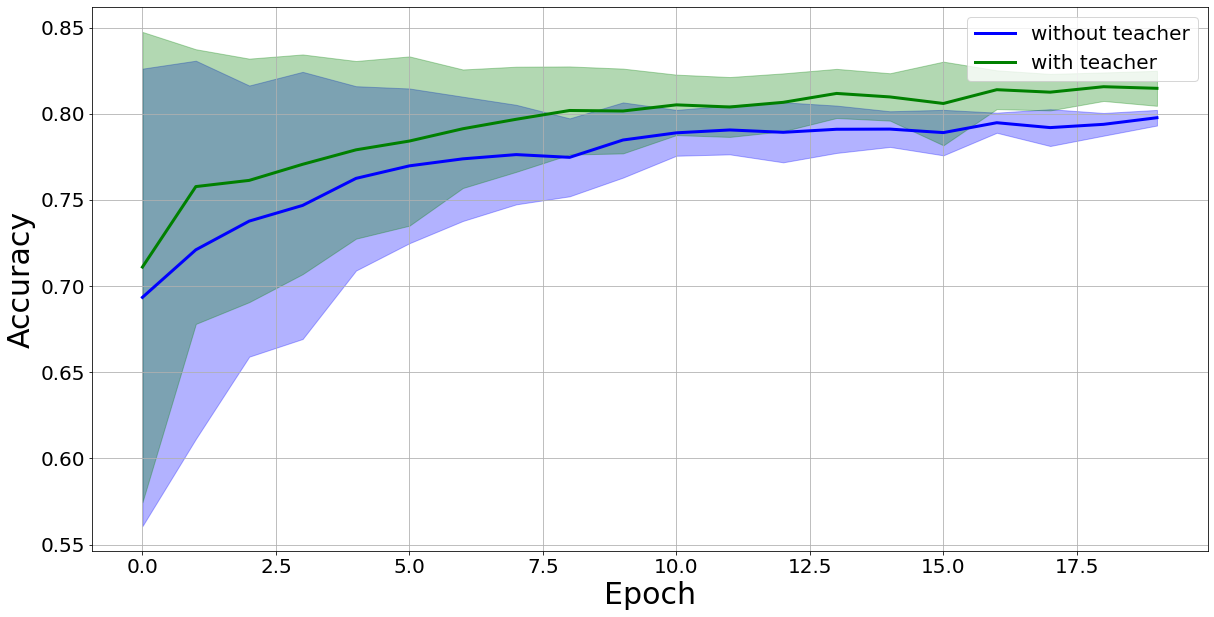
\includegraphics[width=0.45\textwidth]{results/small_acc.png}
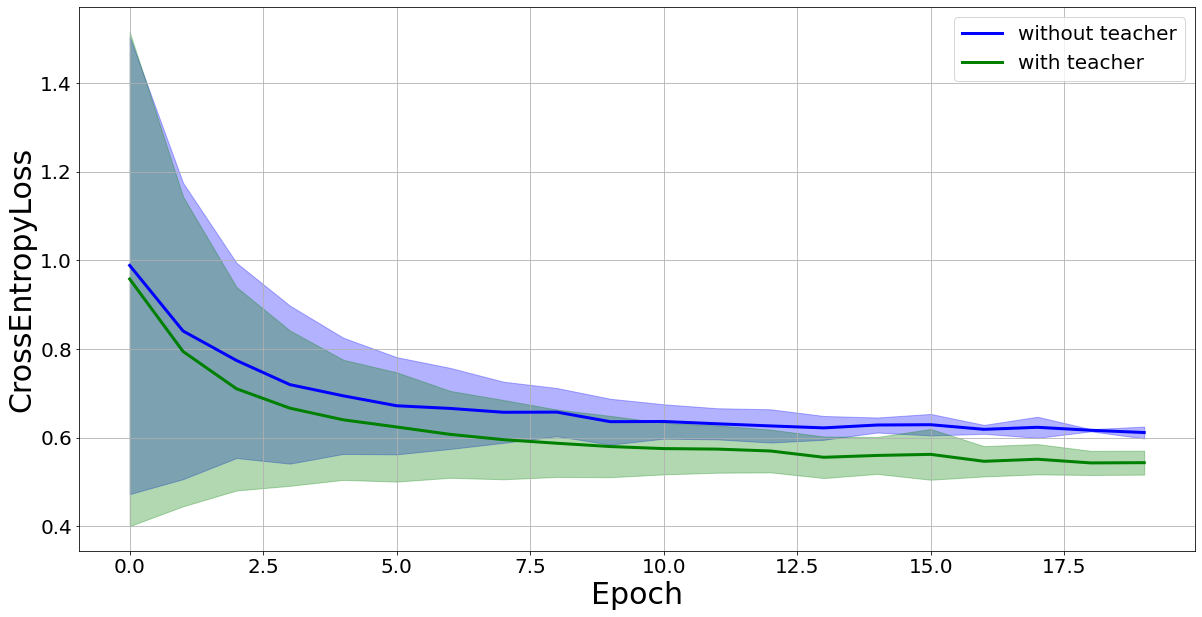
\includegraphics[width=0.45\textwidth]{results/small_loss.png}
\end{figure}

Модель, использующая метки учителя, показывает лучшее значение точности и кросс-энтропийной ошибки, чем модель без учителя.

\end{frame}

%----------------------------------------------------------------------------------------------------------
\section{Анализ дистилляции с нормальным шумом}
\begin{frame}{Анализ дистилляции с нормальным шумом}
\justifying
\begin{enumerate}[1)]
    \item Модель учителя аппроксимирует FashionMNIST-Big с шумом $\mathcal{N}\bigr(0,\frac{1}{10}\bigr)$,
    \item Модель ученика аппроксимирует FashionMNIST-Small без шума.
\end{enumerate}

\par
В качестве отображения $\varphi$ используется нормальный шум.

На графиках показаны метрики точности и кросс-энтропийной ошибки модели ученика.

\begin{figure}[h!]
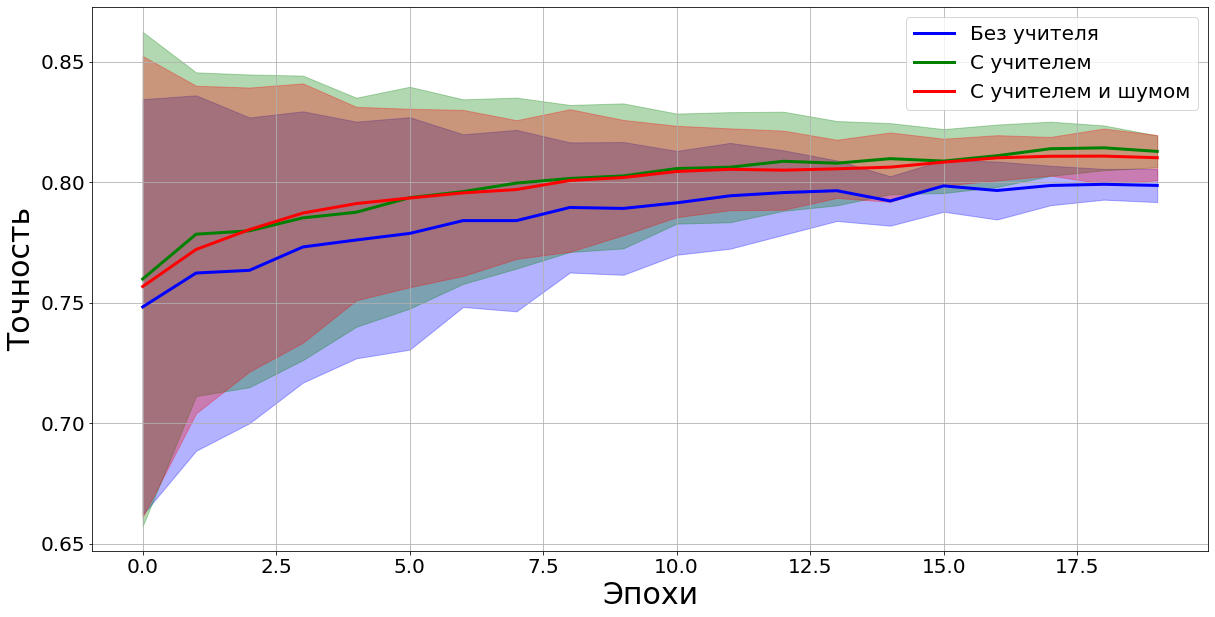
\includegraphics[width=0.45\textwidth]{results/noise_acc.png}
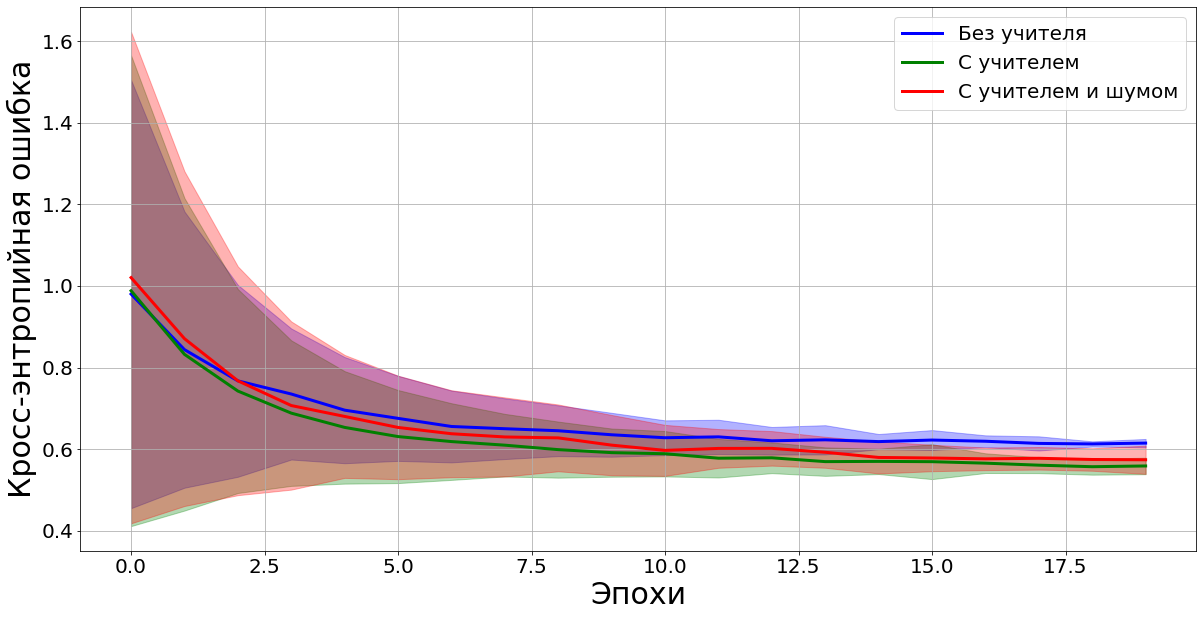
\includegraphics[width=0.45\textwidth]{results/noise_loss.png}
\end{figure}

Модель, использующая метки учителя с применением шума, показывает лучшее значение точности и кросс-энтропийной ошибки, чем модель без учителя.

\end{frame}

%----------------------------------------------------------------------------------------------------------
\section{Анализ дистилляции со сверточным преобразованием}
\begin{frame}{Анализ дистилляции со сверточным преобразованием}
\begin{enumerate}[1)]
    \item Модель учителя аппроксимирует FashionMNIST-Big со сверточным преобразованием с параметром $dilation=2$,
    \item Модель ученика аппроксимирует FashionMNIST-Small без шума.
\end{enumerate}

\par
В качестве отображения $\varphi$ используется сверточное преобразование с $dilation=2$.

На графиках показаны метрики точности и кросс-энтропийной ошибки модели ученика.

\begin{figure}[h!]
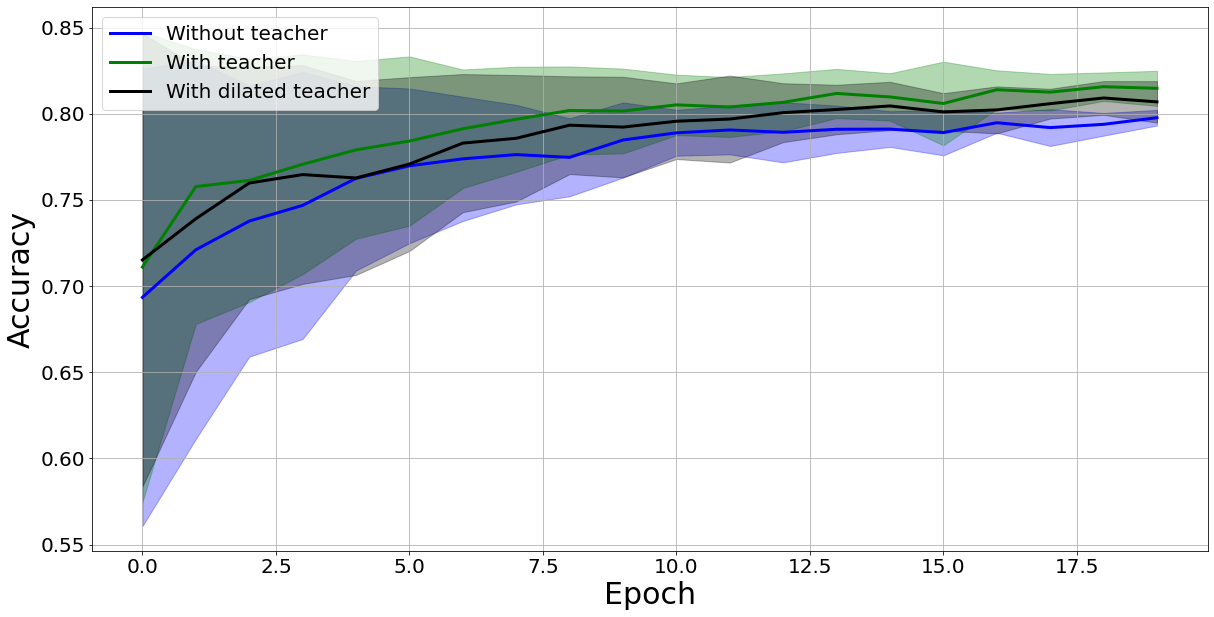
\includegraphics[width=0.45\textwidth]{results/dilation_acc.png}
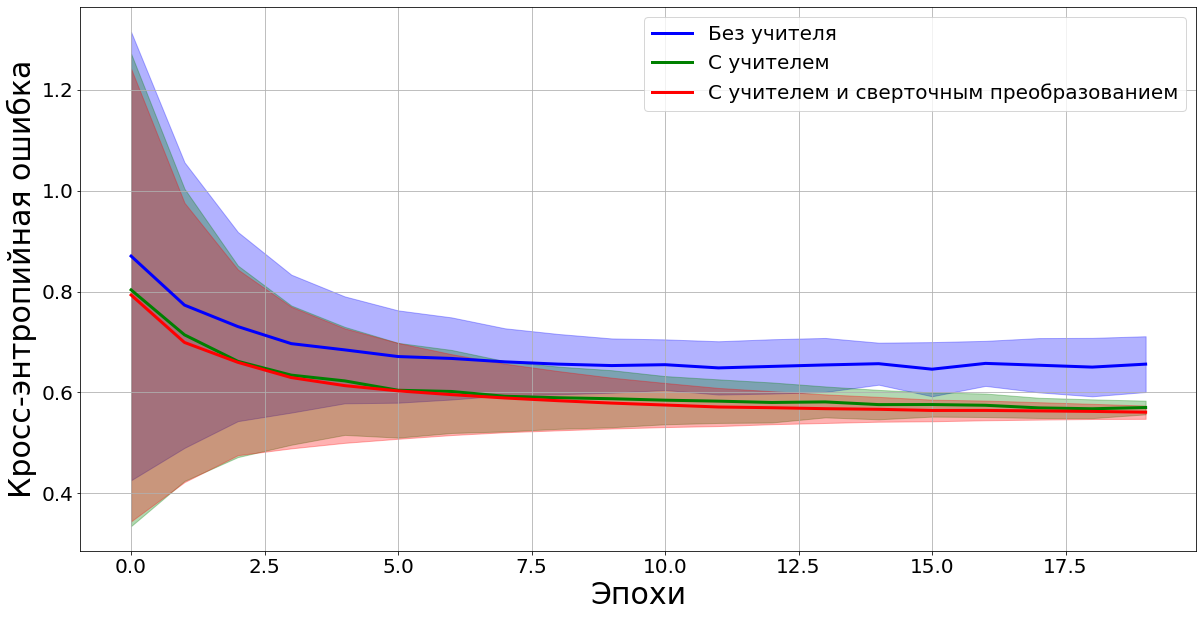
\includegraphics[width=0.45\textwidth]{results/dilation_loss.png}
\end{figure}

Модель, использующая метки учителя со сверточным преобразованием, показывает лучшее значение точности и кросс-энтропийной ошибки, чем модель без учителя.

\end{frame}

%----------------------------------------------------------------------------------------------------------
\section{Вариационный автокодировщик}
\begin{frame}{Вариационный автокодировщик}
\justifying
Отображение $\varphi$ аппроксимируется моделью автокодировщика.

Функция ошибки для обучения автокодировщика:
\[
\begin{aligned}
    \mathcal{L}_{\text{VAE}}(\alpha, \beta)=&\sum\limits_{i=1}^{l}\mathsf{E}_{\mathbf{z}\sim q(\mathbf{z}|\mathbf{x}_{i}, \alpha)}\log{p(\mathbf{x}_{i}|\mathbf{z}, \beta_{MNIST})}\\
    &+\mathsf{E}_{\mathbf{z}\sim q(\mathbf{z}|\mathbf{x}_{i}, \alpha)}\log{p(\mathbf{x}_{i}|\mathbf{z}, \beta_{FashionMNIST})}-\mathsf{KL}(q(\mathbf{z}|\mathbf{x}_{i}, \alpha) || p(\mathbf{z})),
\end{aligned}
\]
где
$p(\mathbf{z})\sim \mathcal{N}(0,\sigma^{2}\mathbf{I})$ --- априорное распределение, $q(\mathbf{z}|\mathbf{x}, \alpha)$ --- вероятностный кодировщик, $p(\hat{\mathbf{x}}|\mathbf{z}, \beta)$ --- вероятностный декодировщик.

Вариационный автокодировщик генерирует новые объекты --- изображения цифр и одежды для одного изображения одежды.

\begin{figure}[h!]
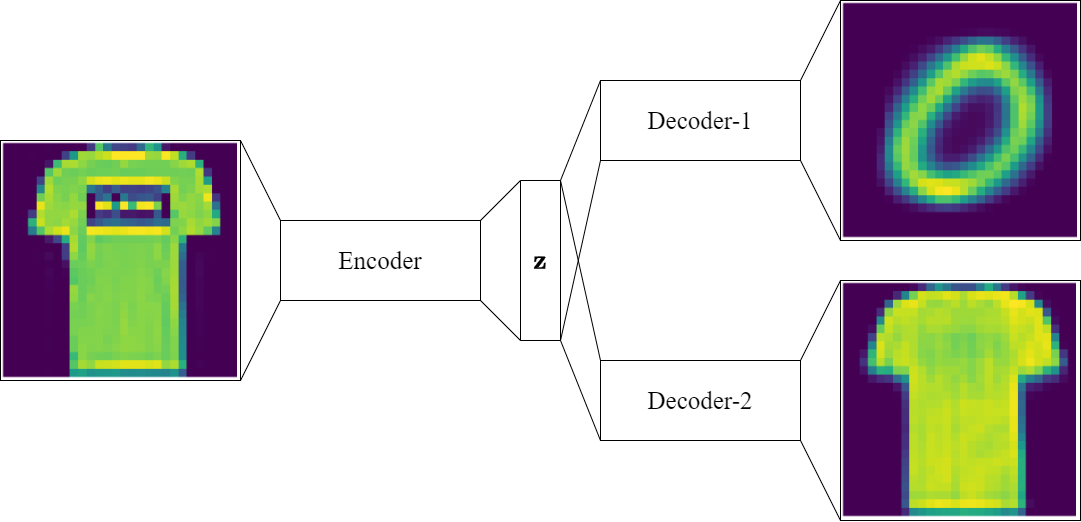
\includegraphics[width=0.45\textwidth]{results/VAE.png}
\end{figure}

\end{frame}

%----------------------------------------------------------------------------------------------------------
\section{Визуализация сгенерированных изображений автокодировщиком}
\begin{frame}{Визуализация сгенерированных изображений автокодировщиком}
\justifying
Проанализируем изменение выхода модели при изменении случайного вектора в скрытом представлении. Для визуализации рассмотрим скрытое представление размерности 2:


\begin{figure}[h!]
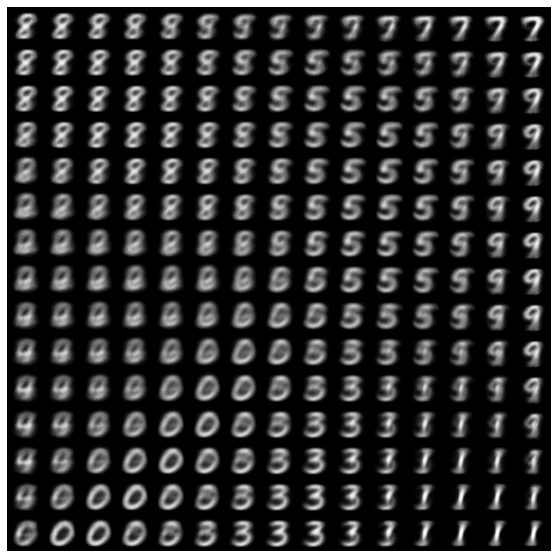
\includegraphics[width=0.45\textwidth]{results/decoder_digits.png}
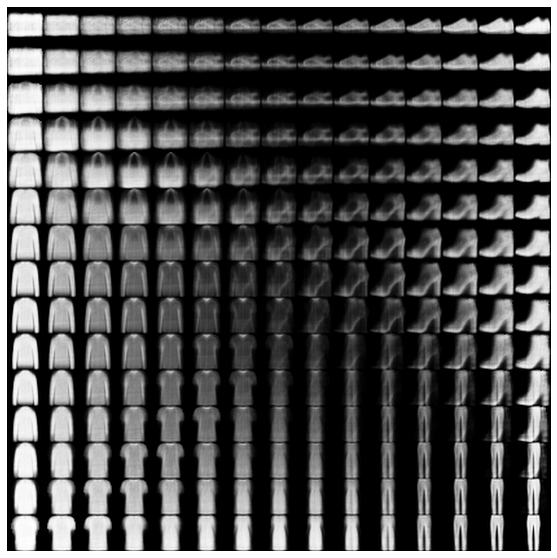
\includegraphics[width=0.45\textwidth]{results/decoder_fashion.png}
\end{figure}

Видно, что классы одежды и цифр соответствуют друг другу.

\end{frame}

%----------------------------------------------------------------------------------------------------------
\section{Анализ дистилляции на основе вариационного автокодировщика}
\begin{frame}{Анализ дистилляции на основе вариационного автокодировщика}
\justifying
\begin{enumerate}[1)]
    \item Модель учителя аппроксимирует MNIST-Big,
    \item Модель ученика аппроксимирует FashionMNIST-Small.
\end{enumerate}

\par
В качестве отображения $\varphi$ используется выход автокодировщика, переводящего изображения одежды в изображения цифр.

На графиках показаны метрики точности и кросс-энтропийной ошибки модели ученика.

\begin{figure}[h!]
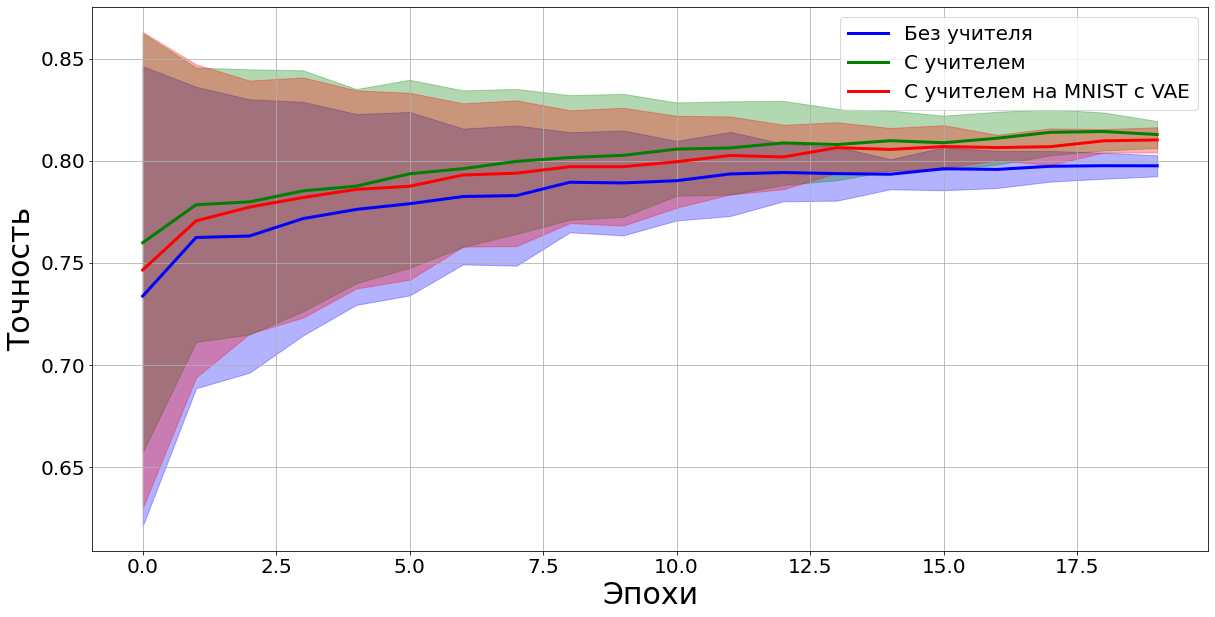
\includegraphics[width=0.35\textwidth]{results/vae_acc.png}
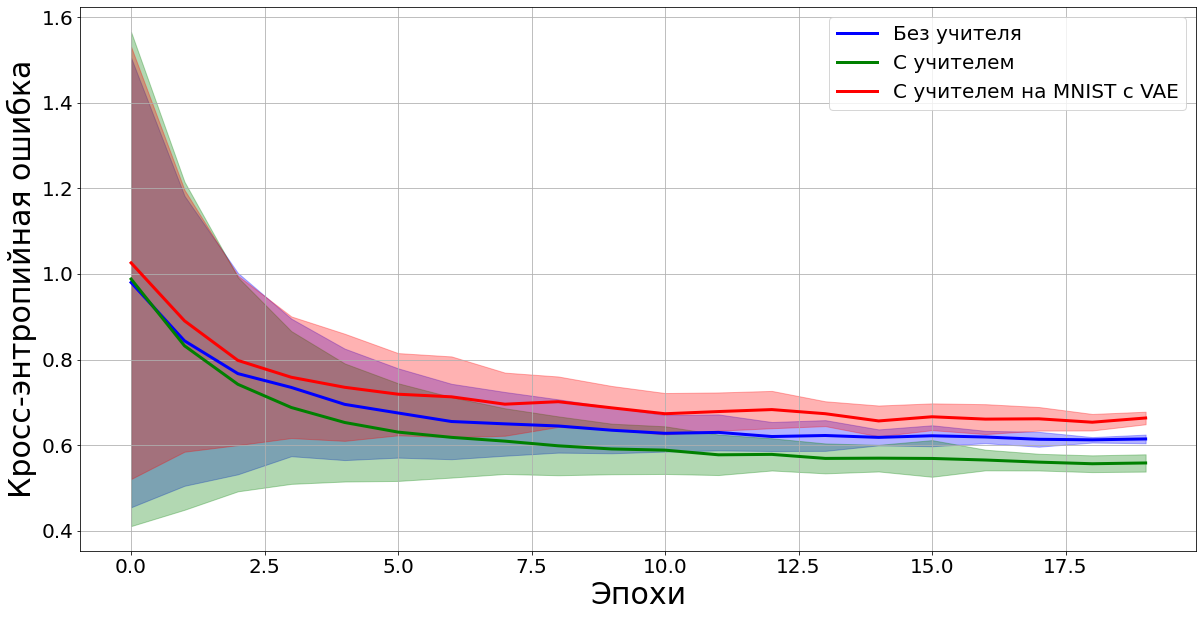
\includegraphics[width=0.35\textwidth]{results/vae_loss.png}
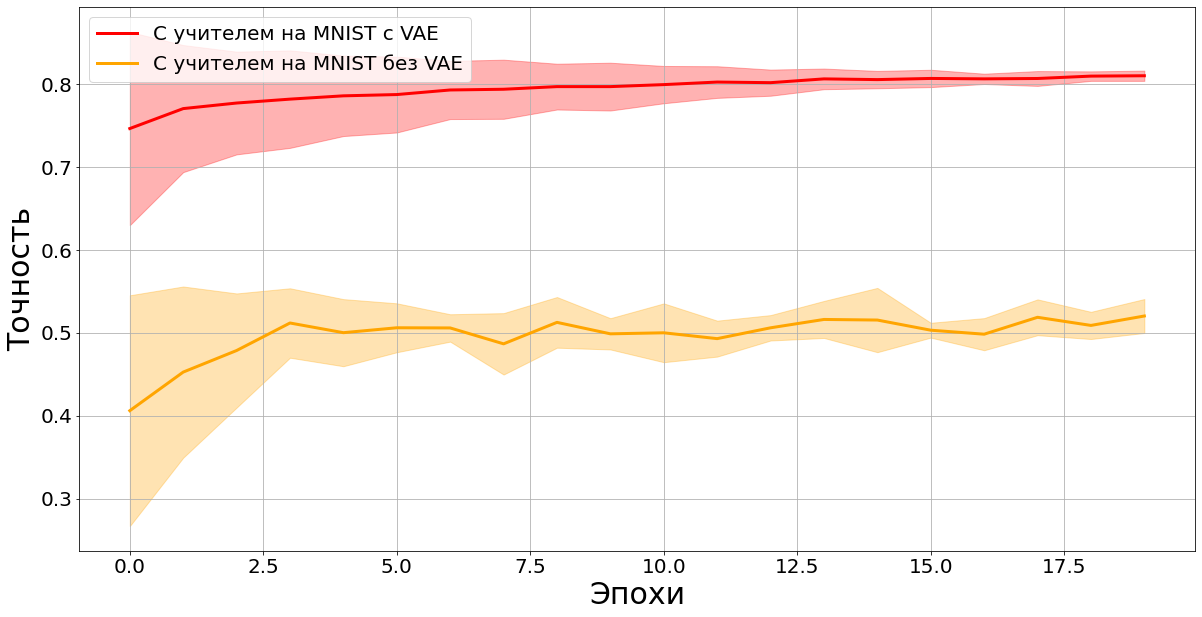
\includegraphics[width=0.35\textwidth]{results/vae_acc_comparison.png}
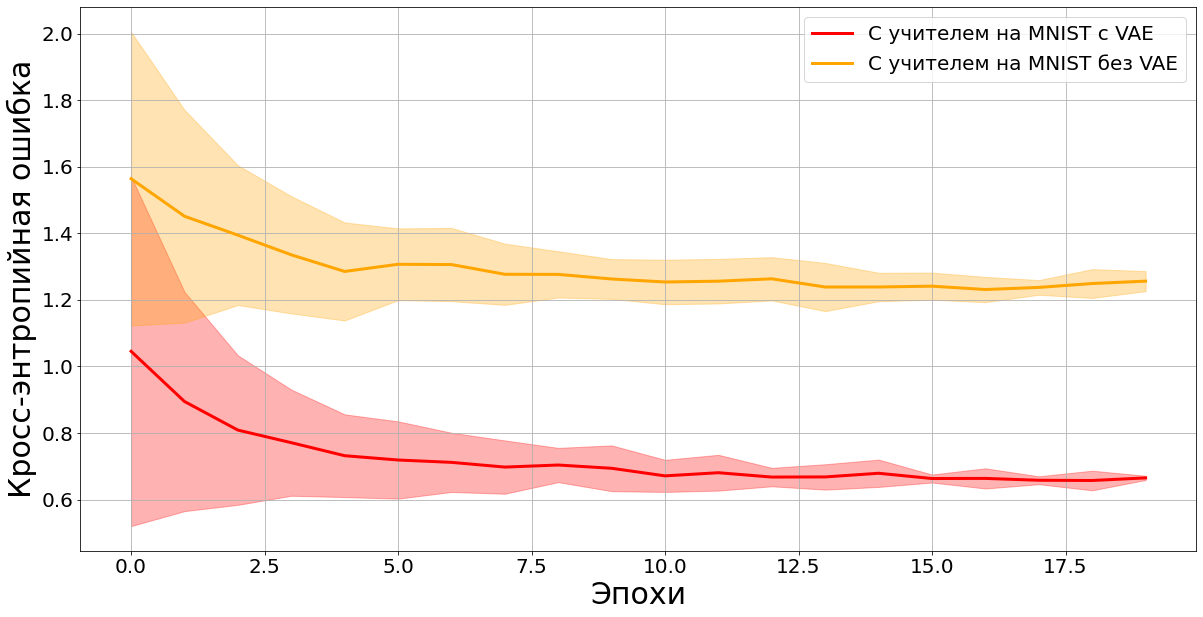
\includegraphics[width=0.35\textwidth]{results/vae_loss_comparison.png}
\end{figure}

Модель, использующая метки учителя с применением вариационого автокодировщика, показывает лучшее значение точности, но большее значение кросс-энтропийной ошибки, чем модель без учителя.

\end{frame}

%----------------------------------------------------------------------------------------------------------
\section{Анализ дистилляции на расширенной синтетически сгенерированной выборке}
\begin{frame}{Анализ дистилляции на расширенной синтетически сгенерированной выборке}
\justifying
На основе выборки FashionMNIST-Small c помощью модели вариационного автокодировщика формируется новая выборка GeneratedMNIST объектов цифр.


\begin{table}[h!t]
\begin{center}
\label{table_1}
\begin{tabular}{|c|c|c|}
\hline
	Выборка & Пояснение &\ Размер выборки\\
	\hline
	\multicolumn{1}{|l|}{GeneratedMNIST-Train}
	& Обучающая часть& 60000\\
	\hline
	\multicolumn{1}{|l|}{GeneratedMNIST-Big}
	& Многоресурсная часть& 59000\\
	\hline
	\multicolumn{1}{|l|}{GeneratedMNIST-Small}
	& Малоресурсная часть& 1000\\
	\hline
	\multicolumn{1}{|l|}{GeneratedMNIST-Test}
	& Тестовая часть& 10000\\

\hline

\end{tabular}
\end{center}
\end{table}

\end{frame}

%----------------------------------------------------------------------------------------------------------
\section{Анализ дистилляции на расширенной синтетически сгенерированной выборке}
\begin{frame}{Анализ дистилляции на расширенной синтетически сгенерированной выборке}
\justifying
\begin{enumerate}[1)]
    \item Модель учителя аппроксимирует GeneratedMNIST-Big,
    \item Модель ученика аппроксимирует FashionMNIST-Small.
\end{enumerate}

\par
В качестве отображения $\varphi$ используется выход вариационного автокодировщика, переводящего изображения одежды в изображения цифр.

На графиках показаны метрики точности и кросс-энтропийной ошибки модели ученика.

\begin{figure}[h!]
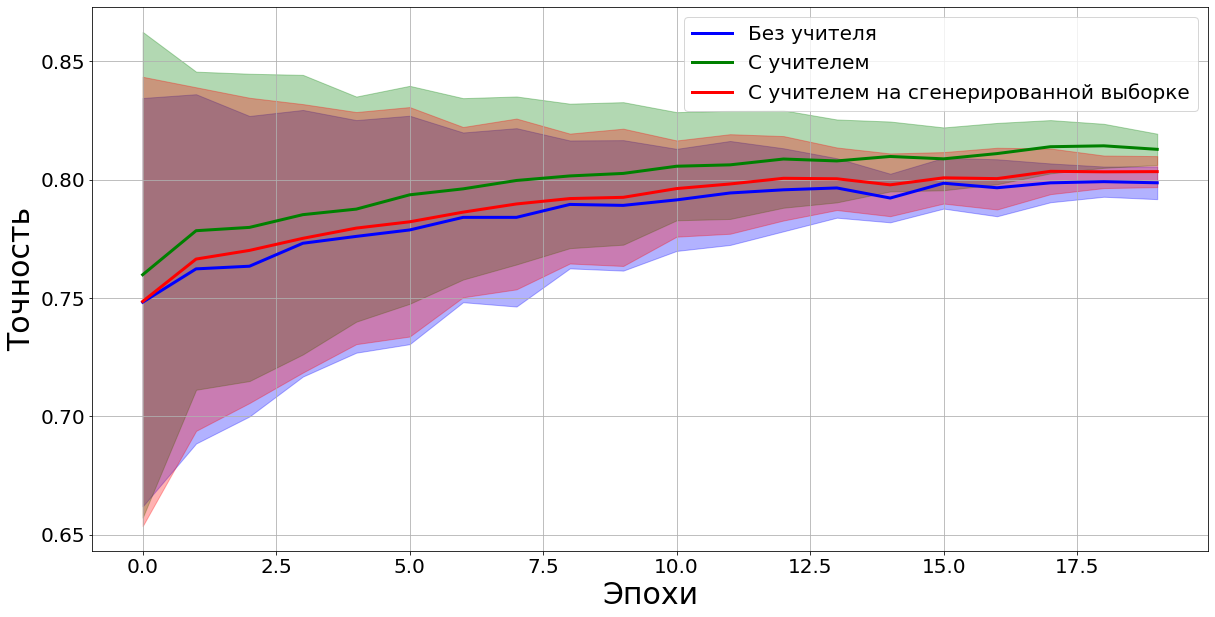
\includegraphics[width=0.45\textwidth]{results/ext_mnist_acc.png}
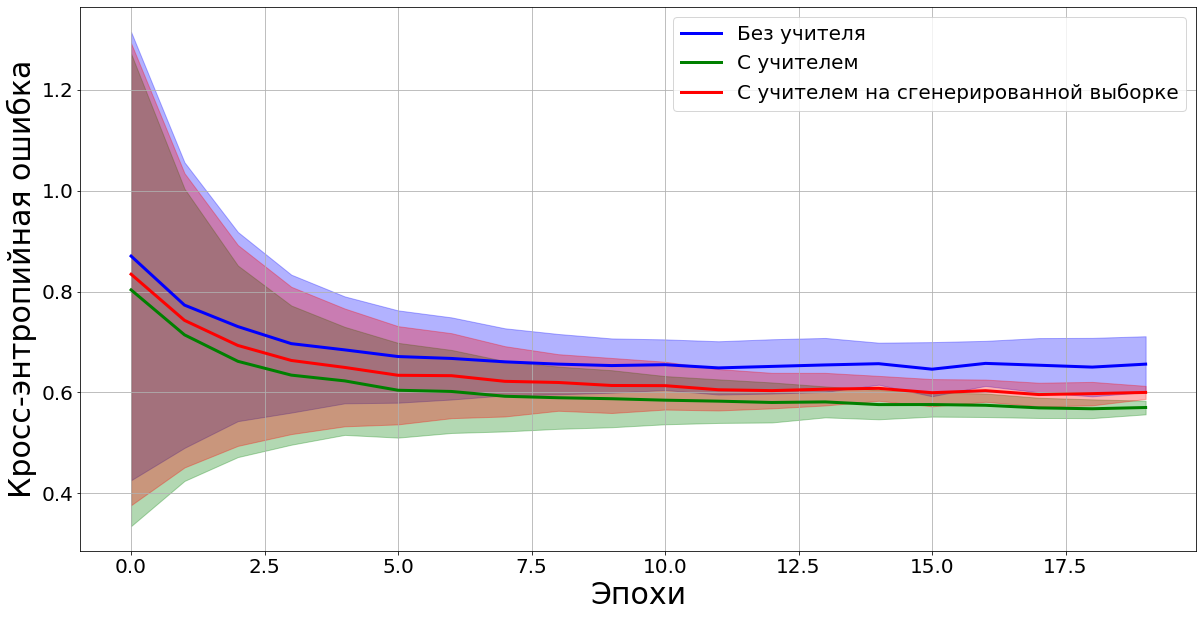
\includegraphics[width=0.45\textwidth]{results/ext_mnist_loss.png}
\end{figure}

Модель, использующая метки учителя с применением вариационого автокодировщика, показывает лучшее значение точности и кросс-энтропийной ошибки, чем модель без учителя.

\end{frame}

%----------------------------------------------------------------------------------------------------------
\section{Выводы}
\begin{frame}{Выводы}
\justifying
	\begin{enumerate}
	\justifying
	    \item Рассмотрена задача снижения сложности модели при ее переносе к новым данным меньшей мощности из близкой генеральной совокупности.
        \item Рассмотрен подход на основе дистилляции моделей глубокого обучения.
        \item Предложен подход для случая, когда модели учителя и ученика заданы на выборках разной мощности с известным отображением между выборками.
        \item Проведен вычислительный эксперимент по анализу качества предложенного метода.
        \item Предложен метод генерации выборки из близкой генеральной совокупности на основе вариационного автокодировщика.
	\end{enumerate}
\end{frame}
%----------------------------------------------------------------------------------------------------------

\end{document}